\section{Подсистема имитационного моделирования}
\indent Подсистема имитационного моделирования -- модуль, производящий моделирование производственных процессов для получения приблизительной оценки времени выполнения набора операций (например карты технологического процесса).\todo{длинное тире}\\
\indent Карта технологического процесса -- документ, предназначенный для операционного описания\todo{?} технологического процесса изготовления или ремонта изделия (составных частей изделия) в технологической последовательности по всем операциям одного вида формообразования, обработки, сборки или ремонта с указанием переходов, технологических режимов и данных о средствах технологического оснащения, материальных и трудовых затратах.

\begin{figure}[ht]
	\centering
	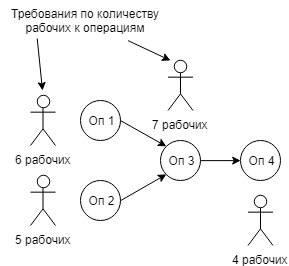
\includegraphics[width=0.6\linewidth]{pics/techMapViz.png}
	\caption{Визуальное представление технологической карты с ограничением по количеству рабочих на операцию}
	\label{fig:map}
\end{figure}

\indent Для имитационного моделирования подсистема преобразует карту технологического процесса в систему неравенств, в которой неизвестными являются времена начала и окончания выполнения операций:

\begin{equation}
	\label{eq:system}
	\begin{cases}
		op1_2 = op1_1 + dur1\\
		op2_2 = op2_1 + dur2\\
		op3_2 = op3_1 + dur3\\
		op4_2 = op4_1 + dur4\\
		op1_2 \leq op3_1\\
		op2_2 \leq op3_1\\
		op3_2 \leq op4_1
	\end{cases}
\end{equation}

\indent Здесь операция обозначается двумя переменными: отметкой начала и конца, которые обозначаются индексами 1 и 2 соответственно.
Первые четыре уравнения задают расчет отметки окончания операции, другие три -- накладывают ограничения на последовательность операций.

\begin{figure}[ht]
	\centering
	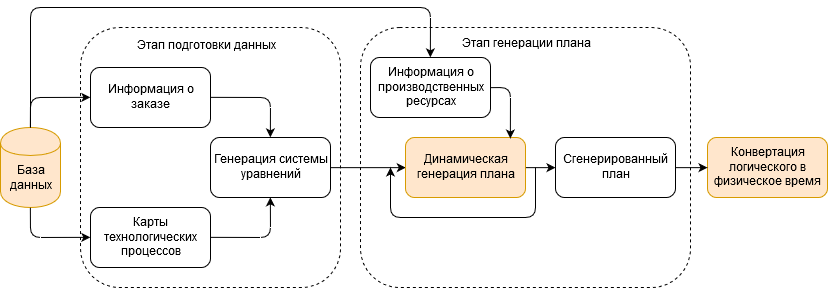
\includegraphics[width=\linewidth]{pics/imcoreDataflow.png}
	\caption{Схема подсистемы имитационного моделирования}
	\label{fig:imcoreFlow}
\end{figure}

\indent В начале работы система выберет одну из независимых переменных (переменные, которые участвуют только в одном неравенстве), например $op1_1$ или $op2_1$ из системы \ref{eq:system} -- список переменных может меняться в зависимости от накладываемых моделью ресурса ограничений (о них речь в следующем разделе).
Система может быть рассчитана тогда, когда можно приравнять любую из независимых переменных к логическому нулю.
Тогда будет произведет подсчет времени окончания выполнения данной операции, то есть по соответствующему уравнению найдет значение окончания операции $op1_2$ или $op2_2$.
Затем по тому же принципу будет выбрано следующее уравнение и так далее пока есть неизвестные переменные.
Когда они закончатся, подсистема завершит свое выполнение, передав результирующие значения и необходимые данные другому модулю, который произведет отображение полученного подсистемой имитационного моделирования числа в физическое время, о чем речь пойдет далее.\todo{обсудить}